\chapter{Metodologia}
\epigraph{\textit{How do you know but ev’ry Bird that cuts the airy way, Is an immense world of delight, clos’d by your senses five?}}{-William Blake}
\section{Motivação}
Como exposto anteriormente na seção \ref{subsection_Conf_Eng}, a confiabilidade de um sistema pode ser quantificada por seu MTTF. Existem diversos fatores que podem afetá-lo e estes podem se manifestar em diversas fases da concepção e operação de um sistema: na variação do processo de fabricação, no design, durante a interação com fatores externos estranhos ao sistema (\textit{p.ex.} descargas elétricas, radiação).

Desta forma, diversos métodos e técnicas são viáveis para mitigar a degradação de transistores nestas fases, combinados ou não. Entretanto, todas estas abordagens alteram, eventualmente, a tensão de operação, a atividade do sistema e indiretamente a temperatura.

Partindo dessa premissa, este trabalho se propõe a averiguar como os parâmetros de tensão e temperatura estão variando ao longo da operação do sistema e investigar a relação destes com a degradação.

\section{Visão geral}
Neste trabalho, os dados de condições ambientais (\textit{p.ex.} tensão e temperatura) auxiliam na criação de um \textit{perfil de operação} para um sistema observado ao longo do tempo. Esse perfil é representado por um conjunto de variações das condições ambientais que, empregadas sobre os dispositivos, contribuem para a degradação e, consequentemente, envelhecimento dos mesmos. Isso nos permite associar de forma única esse perfil a um MTTF.

O MTTF pode ser associado a diferentes eventos dentro do ciclo de vida de um sistema, tais como: tempo médio até o surgimento de falhas permanentes em porções especificas dos circuitos, falhas transitórias e intermitentes, tempo necessário até a falha completa ou parcial de um sistema. Neste trabalho, o MTTF é considerado como sendo o tempo necessário para que um sistema sofra uma degradação alta o suficiente que o force a violar suas especificações de projeto. Em outras palavras, os circuitos não são mais capazes de cumprir suas especificações de temporização.

A partir disso, o \textit{Tempo de Vida Restante} (\textit{i.e. Remaing Useful Lifetime, RUL}) é definido como o tempo remanescente do sistema durante o qual ainda funcionará, antes de falhar \cite{Urmanov2007}. O RUL é, usualmente, determinado pela diferença entre seu tempo de vida atual e seu MTTF. Ao assumir esta proposição, a predição do MTTF através da observação da variação de temperatura $T$, tensão de operação $V$ e da atividade $\alpha$ permite predizer também o RUL.

\begin{figure}[H]
	\center
	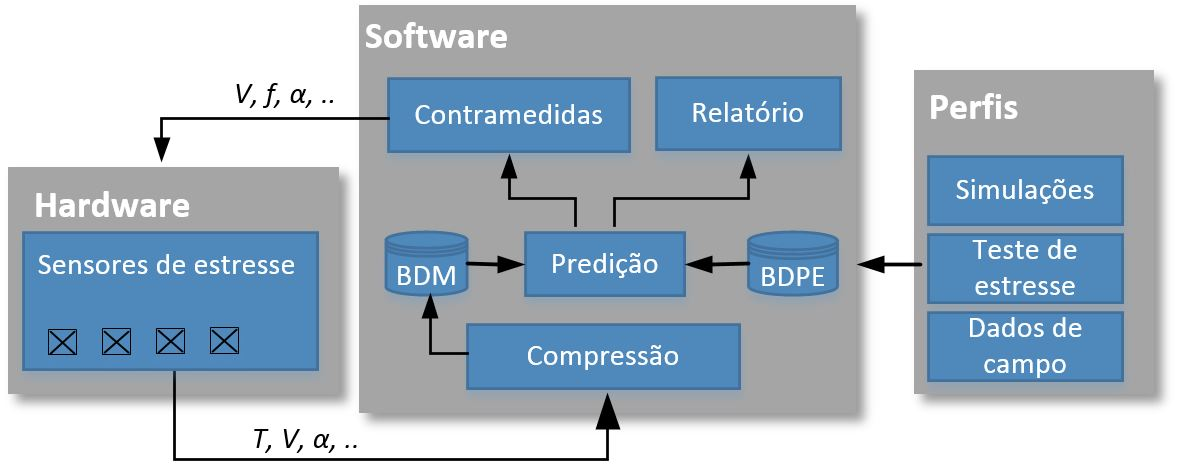
\includegraphics[width=1\textwidth]{images/sistema_proposta_metodologia}
	\caption{Abordagem proposta para análise de envelhecimento.}
	\label{figure:sistema_proposta_metodologia}
\end{figure}

Quais perfis serão definidos e como serão utilizados são decisões que podem ser tomadas pelo projetista durante o projeto. De forma geral, a unidade de \textit{Predição}, ilustrada na figura \ref{figure:sistema_proposta_metodologia}, comunica-se com duas bases de dados: uma responsável por armazenar os perfis \textit{online} medidos pelos sensores e eventualmente comprimidos pela unidade de \textit{Compressão}; e a outra por armazenar perfis pré-existentes que foram criados \textit{offline}, durante o projeto ou atualizados posteriormente, durante a operação do sistema. Essas bases são denominadas, para este trabalho, de Banco de Dados de Medições (BDM) e Banco de Dados de Perfis Envelhecidos (BDPE), respectivamente.

Através de um método de estimativa (que fica a critério do projetista), a unidade de \textit{Predição} estima qual é o tempo de vida restante do sistema e em seguida envia esta informação à unidade de \textit{Contramedidas}. Esta, por sua vez, realiza alguma ação objetivando mitigar a degradação do sistema, quando for o caso. Concomitantemente, essas informações são enviadas a uma unidade de \textit{Relatório}, onde serão armazenadas.

Caso decida por mitigar a degradação, a unidade de Contramedida deve enviar sinais de controle que permitam ao Hardware alterar os parâmetros que estão contribuindo com o envelhecimento do sistema (\textit{p. ex.} tensão de operação, grau de atividade).

A abordagem apresentada acima é generalista e flexível. Isso significa que ela independe de quais parâmetros se deseja obter através dos sensores, de quais métodos sejam utilizados para predição dos MTTFs ou de onde se originam os perfis da BDPE: se são provenientes de simulações, testes de estresse ou dados de campo.

Outra vantagem desta abordagem é a capacidade de popular o banco de dados de perfis com novas observações durante a atual operação do sistema. Uma BDPE que, por exemplo, possuía dados provenientes de simulações \textit{offline} pode, à medida que o sistema envelhece, ter seu conteúdo atualizado com dados de campo, melhorando as estimativas posteriores. Ainda mais: é possível que os modelos utilizados sejam atualizados com melhorias provenientes de otimizações ou até mesmo substituídos por modelos diferentes e melhores.

Posto isso, nas seções subsequentes serão descritas as técnicas e métodos utilizados neste trabalho e utilizará a figura \ref{figure:sistema_proposta_metodologia} como referência.

\section{Sensores}
O uso de sensores para observação de grandezas como temperatura, variações de tensão, grau de atividade e corrente de fuga é bem conhecido e objetivo de inúmeras pesquisas. Diversos deles são projetados especificamente para medir desgastes provenientes dos mecanismos de HCI, BTI e TDDB \cite{Kim2010}\cite{Keane2010}\cite{Kim2008}\cite{Karl2008}, descritos na seção \ref{subsection_Conf_CI}.

Entretanto, neste trabalho é considerado o uso de sensores de estresse para obtenção dos perfis de operação, medindo parâmetros como temperatura, tensão de alimentação ou grau de atividade. Um sensor de atividade realiza o monitoramento das entradas primárias de um sistema ou de uma parte delas para auxiliar na estimativa de estresse. Como exemplo de um sensor de atividade, pode-se utilizar circuitos que observem a variação das entradas e associe a cada transistor a existência ou não de degradação \cite{Baranowski2015}. A figura \ref{figure:monitor_atividades} mostra um exemplo genérico que auxilia o entendimento desta abordagem, onde $E1, E2$ e $E3$ são sinais de entrada que podem alterar o sinal de saída $S$:
\begin{figure}[H]
	\center
	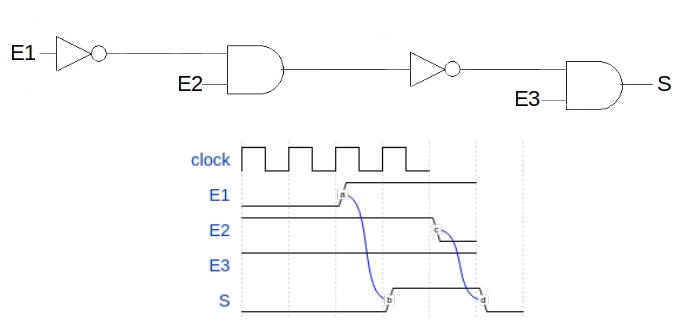
\includegraphics[width=0.7\textwidth]{images/monitor_atividades}
	\caption{Alteração das entradas refletem-se como uma atividade nas portas lógicas.}
		\label{figure:monitor_atividades}
\end{figure}

No exemplo, o sinal da entrada $E1$ é alterado após um período de tempo, mudando o sinal da saída $S$. O mesmo ocorre para a entrada $E2$. Na técnica de monitoramento do grau de atividade, essas alterações podem resultar em uma degradação das portas lógicas que estão presentes no caminho percorrido pelo sinal que vai desde $E1$ até a $S$: duas portas NOT e duas AND2.

Isso significa que, a mudança dos sinais $E1$, $E2$ e $E3$ pode alterar como os transistores de cada porta lógica se comportam (\textit{p.ex.} número de transistores pMOS ativos das portas AND2 do exemplo). Esse comportamento, por sua vez, pode estar associado a um envelhecimento maior ou menor dos transistores decorrentes da degradação por NBTI, por exemplo.

Uma vez determinada essa atividade e a degradação, elas são associadas entre si para que futuras degradações sejam estimadas. O aumento da área total do sistema, decorrente da inserção destes circuitos de monitoramento, é dependente da quantidade de circuitos do sistema a serem monitorados e da precisão desejada na estimativa da degradação \cite{Baranowski2015}.

Já para o caso de sensores de temperatura e tensão de alimentação, a frequência com que essas grandezas variam ao longo do tempo impõem restrições no que se refere ao seu armazenamento, visto que armazenar cada transição de temperatura, por exemplo, exigiria dos sensores ou da unidade de Compressão uma capacidade de armazenamento restritiva. Isto por sua vez aumentaria a área total do sistema, o que pode ser ainda mais restritivo em muitos casos.

Fica então a cargo do projetista escolher qual será a frequência de coleta dos dados ou se será usada alguma métrica que represente a grandeza desejada para um intervalo de medição (p.ex. a temperatura média em um período de tempo $\delta t$). É necessário salientar que esta abordagem incorre na redução de precisão na aferição realizada pelos sensores.

Em contrapartida, a memória necessária para armazenar estas informações é consideravelmente menor. Para este trabalho será considerado que uma métrica (como a média) foi utilizada para descrever as informações de operação do sistema, que posteriormente serão inseridas tanto o BDM quanto no BDPE.
\section{Geração de perfis}
\label{section_obtencao_dados}
No contexto exposto acima, onde um conjunto de sensores amostram condições ambientais, é preciso estabelecer quais informações se deseja representar ao armazenar estas condições. O intuito desta representação é permitir que seja estimado o MTTF, e consequentemente o RUL, de um sistema. 

Para este trabalho são utilizadas a tensão de alimentação $V_{TH}$ e temperatura $T$ como condições ambientais a serem representadas no BDM e BDPE. A literatura e pesquisas exploradas na seção \ref{subsection_estado_da_arte} evidenciam uma forte relação entre $V_{TH}$ e $T$ com os efeitos de degradação explanados na seção \ref{subsection_Conf_CI}.

Considerando que as condições ambientais impostas ao sistema variam com sua operação, podemos exemplificar os valores de temperatura obtidos por um sensor $S_{T,4}$ ao longo de $t$ como mostrado na figura \ref{figure:profile_sets}. Neste período o sistema está operando sob diversas faixas de temperatura $T$, denominadas de \textit{Conjunto 1, Conjunto 2, Conjunto 3, Conjunto 4 e Conjunto 5}. Os sensores serão agrupados pelo seu tipo $k$ (\textit{p.ex.} Temperatura $T$, tensão de alimentação $V$ ou atividade $\alpha$) e denotados por $s_{k,i}$, sendo $i$ o índice de um sensor específico (\textit{p.ex.} 1,\ 2,\ 3,\ \dots).

\textit{Exemplo:} Um sistema possui 6 sensores, sendo dois de temperatura e quatro de tensão de alimentação. Os dois sensores serão denotados por $s_{T,1}$ e $s_{T,2}$. Já os de tensão são denotados como $s_{V,1}$, $s_{V,2}$, $s_{V,3}$ e$s_{V,4}$.

Isso significa que, para cada sensor $s_{k,i}$ existe um vetor $S_{k,i}[\ ]$ com $N$ conjuntos para cada sensor. Um elemento $n$ do vetor $S_{k,i}[\ ]$ quantifica o tempo de permanência do sensor $s_{k,i}$ em uma determinada faixa de valor.
\begin{figure}
\center
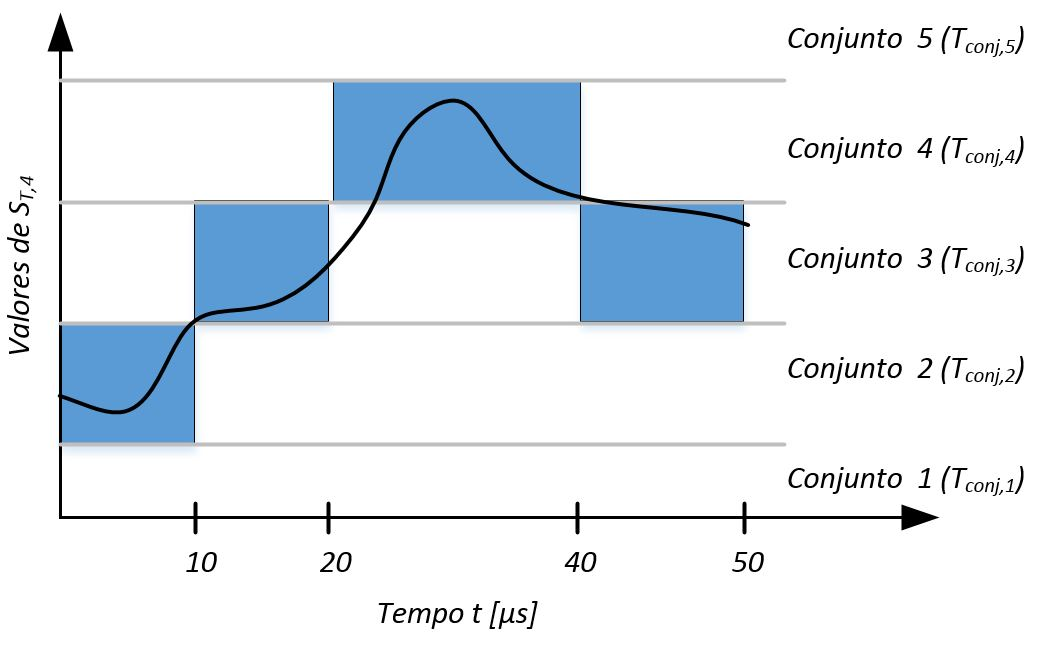
\includegraphics[width=0.8\textwidth]{images/profile_sets}
\caption{Compressão dos dados medidos e representação dos mesmos através de perfis de envelhecimento.}
\label{figure:profile_sets}
\end{figure}

No exemplo mostrado na figura \ref{figure:profile_sets}, para uma medição realizada em um período $\Delta t=10 \mu s$ e um vetor $S_{T,4}[\ ]$ inicialmente vazio, o sensor $s_{T,4}[\ ]$ permanece no conjunto 2 de $t=0 \mu s$ a $t=10 \mu s$. Consequentemente, $S_{T,4}[2]$ recebe o valor 10. Seguindo esta lógica o vetor resultante após 50$\mu s$ é $S_{T,4} = [0,10,20,20,0]$.

A criação dos conjuntos de perfis permite quantificar o estresse aplicado ao sistema e a relação entre os parâmetros dos perfis e o tempo de vida esperado dos circuitos monitorados pelos sensores. Cada perfil é inserido no BDPE conforme exposto na tabela \ref{tb:BDPE}.

Cada linha $w$ contém o percentual de tempo $p_{T(w,x)}$ e $p_{V(w,y)}$ sob os quais um ou mais circuitos monitorados estão submetidos a uma temperatura pertencente ao conjunto $T_{conj,x}$ e uma tensão de alimentação que pertence ao conjunto $V_{conj,y}$ ; sendo $x$ e $y$ os índices dos conjuntos utilizados para descrever o sistema (\textit{p. ex.} $x = 1,\ 2, \ \dots,\ X$ e $y = 1,\ 2,\ \dots,\ Y$).

Como exemplo, a primeira linha ($w=1$) informa que os circuitos monitorados experimentam durante um percentual $p_{T(1,1)}$ de seu tempo de operação $t_{oper}$ uma temperatura pertencente ao conjunto $T_{conj,1}$, um percentual $p_{V(1,1)}$ para uma tensão de alimentação pertencente ao conjunto $V_{conj,1}$ e assim por diante para as colunas subsequentes. Ao final, é esperado que após operar sob estas condições durante $t_{oper}$ seu tempo de vida seja de $MTTF_1$.

\begin{table}[H]
\centering
\begin{tabular}{@{}l|l|l|l|l|l|l@{}}
\toprule
$T_{conj,1}$ & \multicolumn{1}{c}{...} & $T_{conj,X}$ & $V_{conj,1}$ & \multicolumn{1}{c}{...} & $V_{conj,Y}$ & MTTF \\ \midrule
$p_{T(1,1)}$ & ... & $p_{T(1,X)}$ & $p_{V(1,1)}$ & \multicolumn{1}{c}{...} & $p_{V(1,Y)}$ & $MTTF_1$ \\
$p_{T(2,1)}$ & ... & $p_{T(2,X)}$ & $p_{V(2,1)}$ & \multicolumn{1}{c}{...} & $p_{V(2,Y)}$ & $MTTF_2$ \\
\multicolumn{1}{c}{...} & \multicolumn{1}{c}{...} & \multicolumn{1}{c}{...} & \multicolumn{1}{c}{...} & \multicolumn{1}{c}{...} & \multicolumn{1}{c}{...} & \multicolumn{1}{c}{...} \\
$p_{T(M,1)}$ & \multicolumn{1}{c}{...} & $p_{T(M,X)}$ & $p_{V(M,1)}$ & \multicolumn{1}{c}{...} & $p_{V(M,Y)}$ & $MTFF_M$ \\ \bottomrule
\end{tabular}
\caption{Base de Dados de Perfis Envelhecidos}
\label{tb:BDPE}
\end{table}
Aplicando a abordagem anterior à figura \ref{figure:profile_sets} obtemos o excerto representado na tabela \ref{tb:BDPE_reduzida}:
\begin{table}[H]
\centering
\begin{tabular}{@{}l|l|l|l|l|l|l|l|l|l|l@{}}
\toprule
$T_{conj,1}$ & $T_{conj,2}$ & $T_{conj,3}$ & $T_{conj,4}$ & $T_{conj,5}$ & $V_{conj,1}$ & $V_{conj,2}$ & $V_{conj,3}$ & $V_{conj,4}$ & $V_{conj,5}$ & MTTF \\ \midrule
$0$ & $10$ & $20$ & $20$ & $0$ & $0$ & $10$ & $20$ & $20$ & $0$  & $MTTF_1$ \\
\bottomrule
\end{tabular}
\caption{Excerto da BDPE com dados exemplares.}
\label{tb:BDPE_reduzida}
\end{table}
Este exemplo enfatiza a vantagem de perfis granulares (\textit{i.e} que consideram variação nos perfis durante a operação) em comparação a modelos estáticos na obtenção do RUL de um sistema. Estes perfis podem ser obtidos através de simulações de envelhecimento e testes acelerados de estresse. Este trabalho propõe, no capítulo 4, um fluxo de envelhecimento que simule diversos circuitos e extraia esses perfis e utiliza-se de simuladores como os descritos na seção \ref{subsection_Simuladores}.

\section{Métodos de estimativa}
\label{section_metodos_estimativa}
Utilizando ferramentas de simulação e envelhecimento de circuitos aliados a esta abordagem de perfis, é possível estimar o tempo de vida restante de um sistema conhecido. Sendo assim, é necessário determinar a relação entre uma entrada da BDM e a BDPE; e consequentemente o tempo de vida restante. Estas informações podem ser usadas nos métodos de estimativa que serão apresentados a seguir para determinar, aproximadamente, em qual estado o circuito está e o que acontecerá se ele continuar a operar nestas condições.

Um modelo linear geral \cite{McCullagh1984} pode ser utilizado, inicialmente, para estimar a relação entre o atraso de saída e as temperaturas e tensões de entrada; mais especificamente um modelo de regressão linear simples (RLS). Uma RLS ajuda a responder às seguintes perguntas sobre o dado a ser trabalhado \cite{James2013}:
\begin{enumerate}
	\item Existe uma relação entre um conjunto de temperatura $T_{conj,x}$ ou um conjunto de tensão $V_{conj,y}$ e o MTTF?
	\item A relação pode ser descrita linearmente?
\end{enumerate}
A RLS descreve uma variável de resposta $Y$ como dependente de um conjunto de variáveis explicativas $x$ (também chamado de \textit{preditor}) da seguinte forma:
\begin{equation}
\label{eq:regressao_linear_simples}
Y \approx \beta_0+\beta_1X + \epsilon
\end{equation}
sendo $\beta_0$ e $\beta_1$ duas constantes desconhecidas que representam a interceptação da reta com o eixo vertical e a inclinação da mesma, respectivamente. Para representar uma variável ou constante desconhecida e que foi estimada através do modelo, será utilizado o símbolo$\ $ $\hat{}$$\ $. Isso significa que $\hat{y}$ indica uma predição da variável de resposta $Y$ para $X = x$.

Para se estimar $\hat{\beta_0}$ e $\hat{\beta_1}$ é necessário utilizar-se de dados pré-existentes do sistema a ser analisado, obtidos através de simulações, dados de campo ou testes de estresse. Considerando que o projetista possua $n$ observações desse sistema na forma de pares representados por $(x_1,y_1),(x_2,y_2),\dots,(x_n,y_n)$, que consistem de uma medida de $X$ e uma de $Y$, o objetivo da RLS é obter os coeficientes de $\hat{\beta_0}$ e $\hat{\beta_1}$ e um modelo linear que melhor se ajuste ao dados. Ele é descrito como:
\begin{equation}
\label{eq:RLS_estimado}
\hat{y} =\hat{\beta_0}+\hat{\beta_1}x_i
\end{equation}
sendo $i$ o índice do i-ésimo preditor.

O método mais comum de se obter este modelo é através do critério de \textit{mínimos quadrados} \cite{James2013}. Como exemplo, consideremos um conjunto de dados como os mostrados na figura \ref{figure:minimos_quadrados_exemplo} e um modelo representado pela equação \ref{eq:regressao_linear_simples}. Um i-ésimo preditor X, representado por $x_i$, tem como resultado um i-ésimo dado observado $\hat{y}$ para esta equação. 

Entretanto, ao inserir na equação \ref{eq:regressao_linear_simples} um valor de preditor $X = x_i$ cuja resposta $Y$ seja conhecida, o $\hat{y}$ calculado não necessariamente será igual ao $Y$ esperado. A diferença é conhecida como \textit{resíduo} e é representada por $\epsilon$. Assim sendo, o i-ésimo resíduo entre um $Y$ esperado e um $\hat{y}$ estimado é dado por:
\begin{equation}
\label{eq:residuo}
\epsilon_i =  Y_i - \hat{y_i}
\end{equation} 
O critério de \textit{mínimos quadrados} estima $\hat{\beta_0}$ e $\hat{\beta_1}$ de forma a minimizar a \textit{soma dos quadrados dos resíduos} (SQR) que é equivalente a:
\begin{equation}
\label{eq:SQR}
SQR = (y_1-\hat{\beta_0} - \hat{\beta_1}x_1)^2 + (y_2-\hat{\beta_0} - \hat{\beta_1}x_2)^2 + \dots + (y_n-\hat{\beta_0} - \hat{\beta_1}x_n)^2
\end{equation} 
Rearranjando as equações \ref{eq:RLS_estimado} e \ref{eq:SQR}:
\begin{equation}
\label{eq:RLS_coeficientes}
\hat{\beta_1} = \frac{\sum_{i=1}^{n}(x_i-\bar{x})(y_i-\bar{y})}{\sum_{i=1}^{n}(x_i-\bar{x})^2},
\hat{\beta_0} = \bar{y} -\hat{\beta_1}\bar{x} 
\end{equation}
onde $\bar{y}$ e $\bar{x}$ são as médias amostrais de $y$ e $x$, respectivamente.
\begin{figure}
\center
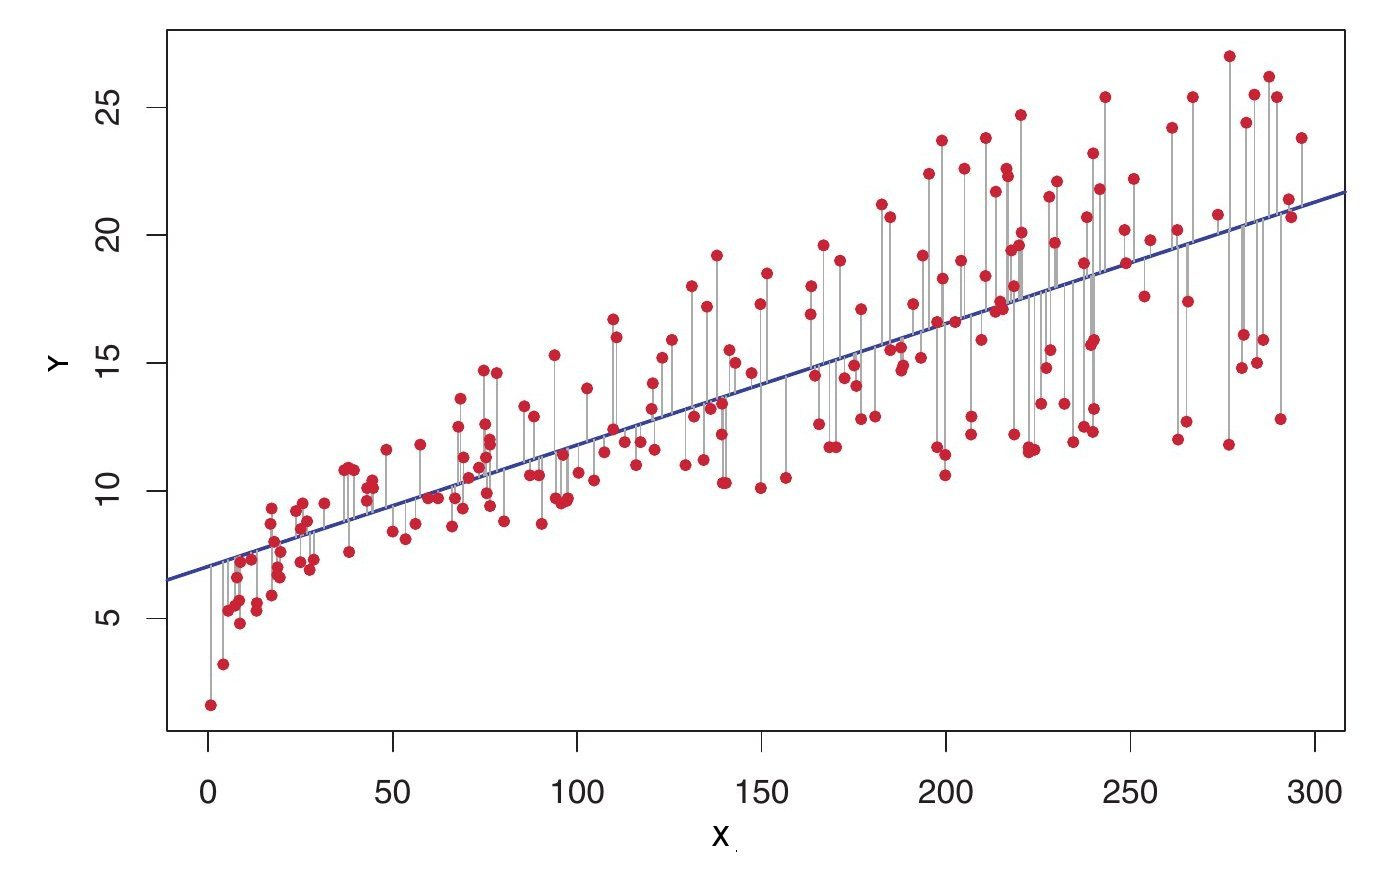
\includegraphics[width=0.8\textwidth]{images/minimos_quadrados_exemplo}
\caption{Modelo linear ajustado a um conjunto de dados de exemplo, representado pela reta azul. Os pontos vermelhos representam os dados coletados e seus respectivos resíduos \cite{James2013}.} 
\label{figure:minimos_quadrados_exemplo}
\end{figure}
Um modelo de RSE descreve de forma simples a relação entre uma grandeza, que funciona como uma variável explicativa, e outra que se deseja estimar, a variável observada.
Entretanto, para o problema que este trabalho tenta solucionar, não é suficiente relacionar somente um preditor a uma observação. Considerando uma BDPE maior, representada pela tabela \ref{tb:regressao_simples_exemplo}, não é possível utilizar somente uma variável explicativa pois o MTTF será função de quatro preditores: $T_{conj,1}=30, T_{conj,2}=50, V_{conj,1}=1.0$ e $V_{conj,2}=1.1$.
\begin{table}[H]
	\centering
	\begin{tabular}{@{}l|l|l|l|l@{}}
		\toprule
		30 & 50 & 1.0 & 1.1 & MTTF \\ \midrule
		13 & 1 & 12 & 2 & 1.2 \\
		7 & 8 & 3 & 12 & 2.7 \\
		1 & 1 & 2 & 2 & 5.3 \\
		5 & 5 & 4 & 7 & 3.5 \\		
		7 & 8 & 4 & 5 & 2.0 \\ \bottomrule
	\end{tabular}
	\caption{Tabela de exemplo para regressão linear simples.}
	\label{tb:regressao_simples_exemplo}
\end{table}
Para o exemplo da tabela \ref{tb:regressao_simples_exemplo}, uma RLS não é capaz de responder os seguintes questionamentos:
\begin{enumerate}
	\item Quão forte é a relação entre conjuntos de $T_{conj,x}$, $V_{conj,y}$ e o MTTF?
	\item Qual dos conjuntos mais contribui para a redução do MTTF? 
\end{enumerate}
Considerando o exemplo da figura \ref{figure:profile_sets} e a subsequente tabela \ref{tb:BDPE_reduzida}, existem dez variáveis explicativas para uma saída desejada, \textit{p. ex.} MTTF. Realizar uma regressão para cada um dos preditores não é satisfatório. Uma melhor abordagem é expandir a RLS para uma Regressão Linear Múltipla (RLM), dando a cada preditor seu próprio coeficiente de inclinação $\beta$. Seu modelo é expresso então por:
\begin{equation}
\label{eq:regressao_linear_multipla}
Y \approx \beta_0+\beta_1X_1 +\dots +\beta_pX_p +\epsilon
\end{equation}
Assim como foi estimado para uma RLS, os coeficientes serão calculados usando o critério de \textit{mínimos quadrados}. Para os valores disponíveis na tabela \ref{tb:regressao_simples_exemplo}, os coeficientes são:
\begin{table}[H]
	\centering
	\begin{tabular}{@{}l|l|l|l|l|l@{}}
		\toprule
		& Interceptação & $T_{conj,1}$ & $T_{conj,2}$ & $V_{conj,1}$ & $V_{conj,2}$ \\ \midrule
		Coeficiente & 5.765 & -0.295 & -0.242 & -0.056 & 0.092 \\ \bottomrule
	\end{tabular}
	\caption{Coeficientes do modelo de RLM para o exemplo da tabela \ref{tb:regressao_simples_exemplo}.}
	\label{tb:regressao_multipla_coeficientes}
\end{table}
Entretanto uma regressão linear múltipla exige uma independência entre essas variáveis explicativas \cite{Chatterjee}, premissa que não podemos garantir dado que os percentuais $p_{T(w,x)}$ e $p_{V(w,x)}$ podem estar correlacionadas. Em adição, a degradação causada pelos conjuntos $T_{conj,x}$ e $V_{conj,x}$ serão dependentes da degradação subsequente dos conjuntos $T_{conj,x-1}$ e $V_{conj,x-1}$.

Ao invés disso, três métodos são propostos: Regressão de mínimos quadrados parciais (Partial Least Square Regression, PLS-R), Distância Euclidiana (DE) e Correlação (COR).
\subsection{Regressão de Mínimos Quadrados Parciais}
\label{subsection_estimativas_PLSR}
A Regressão de Mínimos Quadrados Parciais (PLS-R) é uma técnica que pertence à categoria dos modelos lineares generalizados e que reúne um grupo de algoritmos. Ao contrário da RLM, é menos exigente quanto a existência de correlação entre as variáveis. A PLS-R é classificada como uma abordagem que transforma os preditores e os ajusta a um modelo de mínimos quadrados utilizando-se das variáveis que foram transformadas.

Considere uma combinação linear dos preditores originais $p$ e representada por $Z_1,Z_2,\dots,Z_M$ para $M < p$, onde:
\begin{equation}
Z_m = \sum_{j-1}^{p}\alpha_{jm}X_j
\label{eq:combinacoes_lineares}
\end{equation}
sendo $\alpha_{1m},\alpha_{2m},\dots,\alpha_{pm}$ constantes e $m=1,\dots,M$.

Um modelo de regressão linear pode então ser ajustado por mínimos quadrados e equacionado como:
\begin{eqnarray}
y_i=\theta_0+\sum_{m=1}^{M}\theta_mz_{im}+\epsilon_i, i=1,\dots,n
\label{eq:RLM_PLS}
\end{eqnarray}
Neste caso, os coeficientes de regressão são dados pela constante $\theta$. É possível então definirmos valores de $\alpha$ tais que o modelo para as variáveis transformadas se mostre melhor do que o modelo original.

Por reduzido entende-se que, ao invés de estimarmos $p+1$ coeficientes $\beta_0,\beta_1,\dots,\beta_p$, são estimados $M+1$ coeficientes $\theta_0,\theta_1,\dots,\theta_M$. Dado que $M<p$, como enunciando anteriormente, a dimensão do modelo foi reduzida.

Esta abordagem é compartilhada entre os métodos de compressão. Sumarizadamente, eles possuem duas etapas:
\begin{enumerate}
	\item Obtenção dos preditores transformados $Z_1,Z_2,\dots,Z_M$.
	\item Ajuste do modelo utilizando $M$ preditores.
\end{enumerate}
Entretanto, quais e como os preditores $Z_1,Z_2,\dots,Z_M$ são obtidos varia entre métodos. A proposto em comum é de que, geralmente, uma pequena quantidade deles é suficiente para explicar a variabilidade dos dados originais e sua relação com a resposta. É assumido que a direção para as quais as entradas $X_1,X_2,\dots,X_p$ mostram uma maior variação são as mais associadas à saída Y.

Observando o exemplo da figura \ref{figure:principal_component}, é perceptível que a linha verde segue a direção para a qual as observações mais variam. Esta linha é denominada de \textit{primeiro componente principal}, representado por $Z_1$ e expresso na equação \ref{eq:combinacoes_lineares}.

\begin{figure}[H]
	\center
	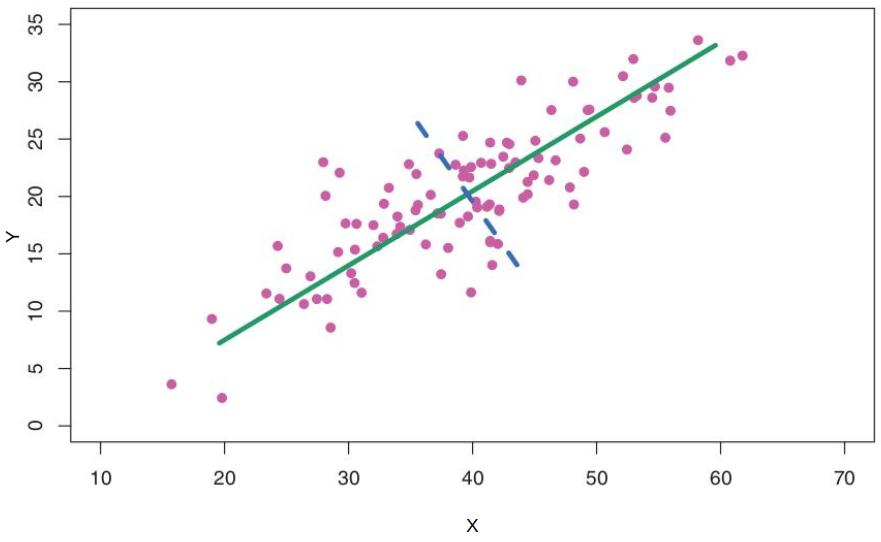
\includegraphics[width=0.8\textwidth]{images/principal_component}
	\caption{Representação de componentes principais. A linha verde representa o primeiro componente e a linha azul o segundo. \cite{James2013}.} 
	\label{figure:principal_component}
\end{figure}

Isso significa que, se os dados observados Y forem projetados nessa reta verde, as projeções apresentarão como resultado a maior variância possível se comparadas com uma projeção em qualquer outra linha que siga a variação dos dados. Em outras palavras, é o vetor que mais próximo está das observações.

Entretanto podemos obter mais componentes que ajudem a descrever os dados. Na figura \ref{figure:principal_component} um \textit{segundo componente principal} $Z_2$ é representado pela linha azul tracejada. Ele é uma combinação linear das variáveis que não estão correlacionadas à $Z_1$ e que, dada esta condição de não-correlação, apresente a maior variância possível.

Como os dados de exemplo da figura \ref{figure:principal_component} são bidimensionais, podemos obter no máximo dois componentes principais. Caso contrário, mais podem ser obtidos e sempre seguindo a premissa de que devem maximizar a variância mas sem estar correlacionados aos componentes anteriores, ou seja, são ortogonais aos mesmos.

Na técnica de \textit{Mínimos Quadrados Parciais} (Partial Least Squares, PLS), o primeiro componente $Z_1$ é obtido através do ajuste de cada $\alpha_{j1}$ da equação \ref{eq:combinacoes_lineares} para que sejam iguais aos coeficientes da regressão linear simples de Y sobre $X_j$ \cite{James2013}. Em seguida, o segundo componente $Z_2$ é computado de forma similar ao $Z_1$, porém utiliza os resíduos obtidos da regressão de $Z_1$.

Os dados residuais são interpretados como sendo a informação remanescente que não foi explicada pelo primeiro componente principal. Os resíduos são então projetados ortogonalmente e o $Z_2$ obtido através de uma regressão linear destes dados.

Essa técnica implica que os dados da BDPE e BDM podem ser reduzidos para uma representação de menor dimensão \cite{Maitra2008}. O PLS tenta maximizar a variância dos estimadores e auxilia a identificar quantos deles são necessários para explicar os dados da BDM e BDPE. É possível então descrever o MTTF de um sistema como uma RLM cujos coeficientes são iguais aos componentes obtidos.

Assim sendo, o MTTF será uma função dessa regressão e pode ser expressada da seguinte forma:
\begin{equation}
MTTF = \hat{y}= \hat{\beta_0}x_0+\hat{\beta_1}x_1+\dots+\hat{\beta_n}x_n
\label{eq:MTTF_estimadores}
\end{equation}
onde $\beta_i$ são o ponto de interceptação da reta e coeficientes da RLM e que ajustam a contribuição dos estimadores $x_i$. A quantidade $i$ de estimadores pode ser determinada pelo projetista, que deve procurar a quantidade de estimadores que melhor explique seus dados. 

\subsection{Distância Euclidiana}
\label{subsection_estimativas_euclidiana}
A Distância Euclideana é definida como a representação da distância entre dois pontos representados no espaço euclideano \cite{Deza2009}. Esta métrica é particularmente útil pois permite uma representação trivial da distância entre dois elementos que se deseja analisar.

Na PLS-R é feita uma estimativa a partir de dados pré-existentes e um modelo linear é obtido. Entretanto, na DE é possível se estimar qual dos perfis $p_{T(w,x)}$ e $p_{V(w,y)}$ pré-existentes na BDPE mais se aproxima do perfil medido pelos sensores. Essa proximidade é dada pela distância euclidiana.

A distância $d(a,b)$ entre duas séries de pontos $a=(a_1,a_2,\dots,a_N)$ e $b=(b_1,b_2,\dots,b_N)$ com N valores cada pode ser representada pela expressão seguinte:

\begin{equation}
d(a,b)=\sqrt{\sum_{i=1}^{N}(a_i-b_i)^2}
\label{eq:dist_euclideana}
\end{equation}

Para a estimativa do MTTF, é necessário calcular a distância entre cada entrada da BDPE e o perfil obtido pelos sensores. Usando como exemplo a BDPE representada na tabela \ref{tb:regressao_simples_exemplo}, que possui 4 dimensões para suas variáveis explicativas, as distâncias euclideanas para um perfil dado, por exemplo, por $S_{T,4} = [3,8]$ e $S_{V,4} = [9,6]$ são dadas como:

\begin{align}
d(a_1,b_1) = \sqrt{(13-3)^2+(1-8)^2+(12-9)^2+(2-6)^2} = 13.19 \\
d(a_2,b_2) = \sqrt{(7-3)^2+(8-8)^2+(3-9)^2+(12-6)^2} = 9.38 \\
d(a_3,b_3) = \sqrt{(1-3)^2+(1-8)^2+(2-9)^2+(2-6)^2} = 10.86 \\
d(a_4,b_4) = \sqrt{(5-3)^2+(5-8)^2+(4-9)^2+(7-6)^2} = 6.24 \\
d(a_5,b_5) = \sqrt{(7-3)^2+(8-8)^2+(4-9)^2+(5-6)^2} = 6.48
\end{align}

Logo, o perfil de menor distância euclidiana dentre os armazenados na BDPE é o quarto. Consultando a tabela \ref{tb:regressao_simples_exemplo}, o MTTF pertencente à entrada da BDPE que possui a menor distância euclideana é utilizado então para mensurar o tempo de vida restante do sistema. No exemplo fictício desta tabela é estimado que o $MTTF=3.5$.
\subsection{Correlação}
\label{subsection_estimativas_correlacao}

Um terceiro método proposto foi a utilização da Correlação, que essencialmente mostra a dependência e associação entre duas ou mais variáveis \cite{Rodgers1988}. Para identificar uma possível relação entre os dados a serem analisados é definido um \textit{coeficiente de correlação}. É de suma importância salientar que esta métrica não necessariamente implica em causalidade.

Existem diferentes métodos para análise de correlação. Entre eles existe a \textit{Correlação r de Pearson} (CP), também conhecida como \textit{correlação paramétrica}. Ela calcula a dependência linear entre duas variáveis X e Y, um coeficiente cuja representação simbólica é $r$, e que varia entre $+1$ e $-1$. Um valor $r$ que se aproxima cada vez mais de $\pm1$ é interpretado como um grau de associação ``perfeita'' entre duas variáveis. Caso $r$ se aproxime de $0$, é dito que não há correlação ou ela é fraca.

A sinalização $\pm$ indica apenas a direção da correlação, sendo positiva para ``$+$'' e negativa para ``$-$''. Isso significa que em uma correlação positiva, quando uma das variáveis cresce ou decresce em valor, a outra variável acompanha o mesmo sentido de acréscimo ou decréscimo. O contrário pode ser dito da correlação negativa.
A correlação entre dois vetores $x$ e $y$ é quantificada pelo seu coeficiente $r_{x,y}$ e pode ser descrito por:

\begin{align}
r_{x,y}= \frac{\sum_{i=1}^{n}(x-\bar{x})(y-\bar{y})}{\sqrt{\sum_{i=1}^{n}(x-\bar{x})^2 \sum_{i=1}^{n}(y-\bar{y})^2}} \\
r_{x,y}=\frac{cov(x,y)}{\sigma_x,\sigma_y}
\label{eq:correlacao}
\end{align}

onde $cov$ é a covariância; $\bar{x}$ e $\bar{y}$ são as médias de $x$ e $y$; $n$ é o tamanho desses vetores e $\sigma$ é o desvio-padrão da série \cite{Chatterjee}.

Considerando a tabela \ref{tb:regressao_simples_exemplo}, um perfil de interesse dado por $S_{T,4} = [3,8]$ e $S_{V,4} = [9,6]$, os coeficientes de correlação $r$ entre cada perfil da tabela e o perfil de interesse é:
\begin{equation}
r = [-0.2963478, -0.3748790,  0.4364358, -0.3504383, -0.3450328]
\end{equation}
Estamos interessados no resultado com maior correlação dentre eles, no caso $r_4=0.4364358$. Esse coeficiente corresponde à correlação do 3º perfil da nossa tabela de exemplo, cujos valores das variáveis estimativas são $S_{T,4} = [3,8]$, $S_{V,4} = [9,6]$ e seu $MTTF=5.3$.

Em suma, é realizado o cálculo da correlação entre o perfil medido e a as entradas da BDPE, encontrando-se aí a entrada de menor correlação e seu respectivo MTTF.
